
\subsection{Resumen enunciado}


%\bfseries{\color{red} Enunciado:}

\normalfont

Este TP consiste en realizar un pequeño estudio del movimiento de un ascensor, figura~\figref{fig:fig_elevator}, intentando utilizar valores realistas para los parámetros a fin de obtener las expresiones para la posición, $x_{(t)}$, la velocidad, $v_{(t)}$ y la aceleración, $a_{(t)}$. Luego estas expresiones se utilizarán para aplicar un método numérico de nuestra implementación, Newton-Raphson en este caso.





\subsection{Planteo}

El planteo implica asumir ciertas cosas acerca del ascensor, realizando el análisis para el movimiento ascendente, en particular se debe analizar, la altura de un piso, que asumimos ser igual para todos los pisos, siendo en todos por lo tanto el mismo problema, la masa de la cabina y los pasajeros, el tiempo de viaje máximo (se da a máxima carga), la máxima aceleración, y la máxima velocidad, asumimos también por simplicidad que la fuerza que se imprime a la cabina varía linealmente con el tiempo, esto es planteado así en el enunciado. Todas estos parámetros se obtuvieron de normas locales,\citelink{camaradeascensores}, e internacionales, \citelink{elevatorworld}, y de algunos ejemplos de ascensores residenciales comerciales.



%%\begin{figure}[!h] %htb
\begin{wrapfigure}{r}{0.5 \linewidth}
\begin{center}
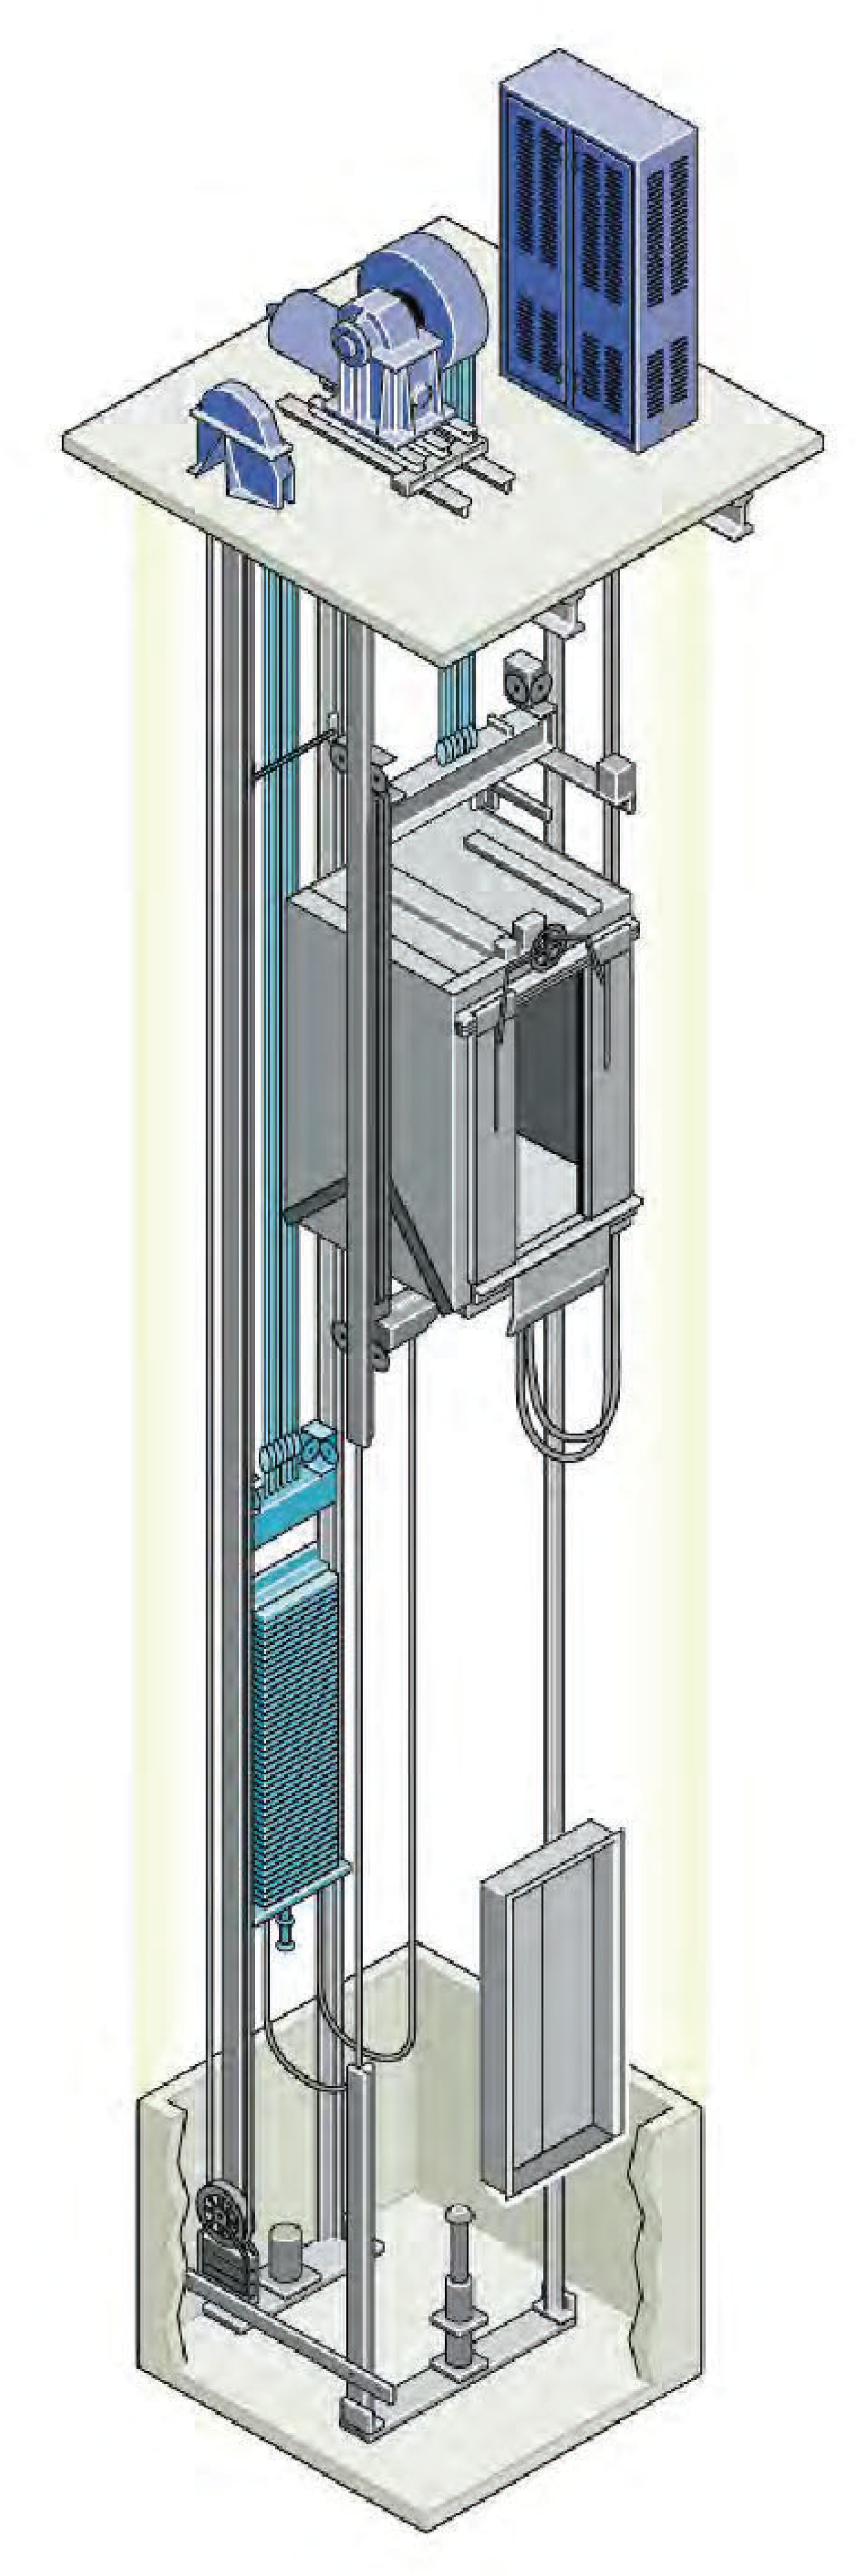
\includegraphics[width=0.35 \linewidth, keepaspectratio=true]{img/diagrams/elevator.png} %% , angle=90 trim={<left> <lower> <right> <upper>}
\caption{\label{fig:fig_elevator} \footnotesize{Ascensor electromecánico.}}
\end{center}
\end{wrapfigure}
%%\end{figure}

En general las normas especifican para la máxima aceleración posible $8 \si[per-mode=symbol]{\meter\per\second\squared}$, la masa de cada persona debe tomarse en promedio como de $75 \si[per-mode=symbol]{\kilogram}$, la masa de la cabina depende del ascensor en cuestión, se tomó un modelo para $12$ personas, con una cabina de masa igual a $450 \si[per-mode=symbol]{\kilogram}$, esto determina la masa máxima de carga en $1350 \si[per-mode=symbol]{\kilogram}$ y la mínima en los $450 \si[per-mode=symbol]{\kilogram}$ de la cabina vacía. Se toman $t_{f} = 3 \si[per-mode=symbol]{\second}$ como el máximo tiempo de tránsito entre pisos, caso que se daría a máxima carga, y se toma la altura entre pisos como, $h_{f} = 4 \si[per-mode=symbol]{\meter}$, el cual es un valor posible en ascensores residenciales, dentro de todo un rango posible. \\
Otras condiciones a tener en cuenta en el planteo, son que se parte de la posición inicial $x_{\left(0\right)} = 0 \si[per-mode=symbol]{\meter}$, se llega a la posición final, $x_{\left( t_{f} \right)} = h_{f}$ y además para la velocidad debe ser, $v_{\left(0\right)} = 0 \si[per-mode=symbol]{\meter\per\second}$ y $v_{\left( t_{f} \right)} = 0 \si[per-mode=symbol]{\meter\per\second}$

\clearpage

De la física del problema se obtienen las expresiones, \eqref{eqn:position}, \eqref{eqn:velocity} y \eqref{eqn:acceleration}, para la posición, velocidad y aceleración, respectivamente.

\begin{equation}
x_{(t)} = A \cdot t^{3} + B \cdot t^{2} + C \cdot t + D
\label{eqn:position}
\end{equation}

\begin{equation}
v_{(t)} = 3 \cdot A \cdot t^{2} + 2 \cdot B \cdot t + C
\label{eqn:velocity}
\end{equation}

\begin{equation}
a_{(t)} = 6 \cdot A \cdot t + 2 \cdot B \cdot
\label{eqn:acceleration}
\end{equation}


Las constantes $A$, $B$, $C$ y $D$ se obtienen de las condiciones y parámetros mencionados anteriormente para el caso de máxima carga, $n_{personas} = 12$, para el caso extremo de mínima carga se asigna la máxima aceleración y se ajusta el tiempo de transito e iterativamente se obtienen las expresiones correspondientes a media carga respetando los parámetros elegidos. Planteando para media carga, se obtiene el siguiente sistema de ecuaciones:

\begin{equation}
 \begin{cases}
 4 = & 27A + 9B\\
 0 = & 27A + 6B \\
 0 = & C\\
 0 = & D 
 \end{cases} 
\end{equation}


Se obtiene $t_{f} = 3 \si[per-mode=symbol]{\second}$, $A = -0.2963 \si[per-mode=symbol]{\meter\per\second\cubed}$ y $B = 1.3333 \si[per-mode=symbol]{\meter\per\second\squared}$, con lo que nos queda:


\begin{empheq}[box={\mybluebox[5pt]}]{equation}
 \begin{cases}
 {x_{cmax}}_{\left( t \right)} = & -0.2963 \si[per-mode=symbol]{\meter\per\second\cubed} \cdot t^3 + 1.3333 \si[per-mode=symbol]{\meter\per\second\squared} \cdot t^2  \\
 {v_{cmax}}_{\left( t \right)} = & -0.8889 \si[per-mode=symbol]{\meter\per\second\cubed} \cdot t^2 + 2.6667 \si[per-mode=symbol]{\meter\per\second\squared} \cdot t\\
 {a_{cmax}}_{\left( t \right)} = & -1.7778 \si[per-mode=symbol]{\meter\per\second\cubed} \cdot t + 2.6667 \si[per-mode=symbol]{\meter\per\second\squared}
 \end{cases} 
\end{empheq}

Para el caso de mínima carga, $n_{personas} = 0$ (con la cabina vacía), asumiendo que la fuerza inicial es la misma y que la máxima aceleración debe ser de $8 \si[per-mode=symbol]{\meter\per\second\squared}$, ahora para una masa total de $450 \si[per-mode=symbol]{\kilogram}$, tenemos:

\begin{equation}
 \begin{cases}
 4 = & A \cdot t_{f}^3 + 4 \cdot t_{f}^2 \\
 0 = & 3A \cdot t_{f}^2 + 8 \cdot t_{f} \\
 \end{cases} 
\end{equation}


Se obtiene $A = -1.5396 \si[per-mode=symbol]{\meter\per\second\cubed}$ y $t_{f} = 1.7321 \si[per-mode=symbol]{\second}$, con lo que nos queda:


\begin{empheq}[box={\mybluebox[5pt]}]{equation}
 \begin{cases}
 {x_{cmin}}_{\left( t \right)} = & -1.5396 \si[per-mode=symbol]{\meter\per\second\cubed} \cdot t^3 + 4 \si[per-mode=symbol]{\meter\per\second\squared} \cdot t^2  \\
 {v_{cmin}}_{\left( t \right)} = & -4.6188 \si[per-mode=symbol]{\meter\per\second\cubed} \cdot t^2 + 8 \si[per-mode=symbol]{\meter\per\second\squared} \cdot t\\
 {a_{cmin}}_{\left( t \right)} = & -9.2376 \si[per-mode=symbol]{\meter\per\second\cubed} \cdot t + 8 \si[per-mode=symbol]{\meter\per\second\squared}
 \end{cases} 
\end{empheq}


Por último para el caso de carga media, $n_{personas} = 6$, nuevamente con la misma fuerza inicial y ahora con una masa total de $900 \si[per-mode=symbol]{\kilogram}$, tenemos:

\begin{equation}
 \begin{cases}
 4 = & A \cdot t_{f}^3 + 2 \cdot t_{f}^2 \\
 0 = & 3A \cdot t_{f}^2 + 4 \cdot t_{f} \\
 \end{cases} 
\end{equation}


Se obtiene $A = -0.5443 \si[per-mode=symbol]{\meter\per\second\cubed}$ y $t_{f} = 2.4495 \si[per-mode=symbol]{\second}$, con lo que nos queda:


\begin{empheq}[box={\mybluebox[5pt]}]{equation}
 \begin{cases}
 {x_{cmin}}_{\left( t \right)} = & -0.5443 \si[per-mode=symbol]{\meter\per\second\cubed} \cdot t^3 + 2 \si[per-mode=symbol]{\meter\per\second\squared} \cdot t^2  \\
 {v_{cmin}}_{\left( t \right)} = & -1.6329 \si[per-mode=symbol]{\meter\per\second\cubed} \cdot t^2 + 4 \si[per-mode=symbol]{\meter\per\second\squared} \cdot t\\
 {a_{cmin}}_{\left( t \right)} = & -3.2658 \si[per-mode=symbol]{\meter\per\second\cubed} \cdot t + 4 \si[per-mode=symbol]{\meter\per\second\squared}
 \end{cases} 
\end{empheq}



\subsection{Planteo extra - Dimensionamiento de los frenos del ascensor}

Para el dimensionamiento del frenado del ascensor, partimos de suponer que el ascensor cae de la posición de reposo, moviéndose en caída libre,  $a_{\left( t \right)} = g$, durante los $0.8 \si[per-mode=symbol]{\second}$ que le toma al sistema detectar el fallo, y dimensionando el frenado de tal forma de limitar la aceleración, el sistema solo logra detener totalmente el ascensor si este se encuentra a una altura mínima determinada, el sistema se completa con un sistema de topes hidráulicos o buffers, figura~\figref{fig:fig_elevator_buffer}, que absorben la energía restante cuando la cabina del ascensor los golpea, este tipo de buffers son obligatorios en ascensores que desarrollan velocidades que cruzan un umbral establecido por normas.


%%\begin{figure}[!h] %htb
\begin{wrapfigure}{l}{0.5 \linewidth}
\begin{center}
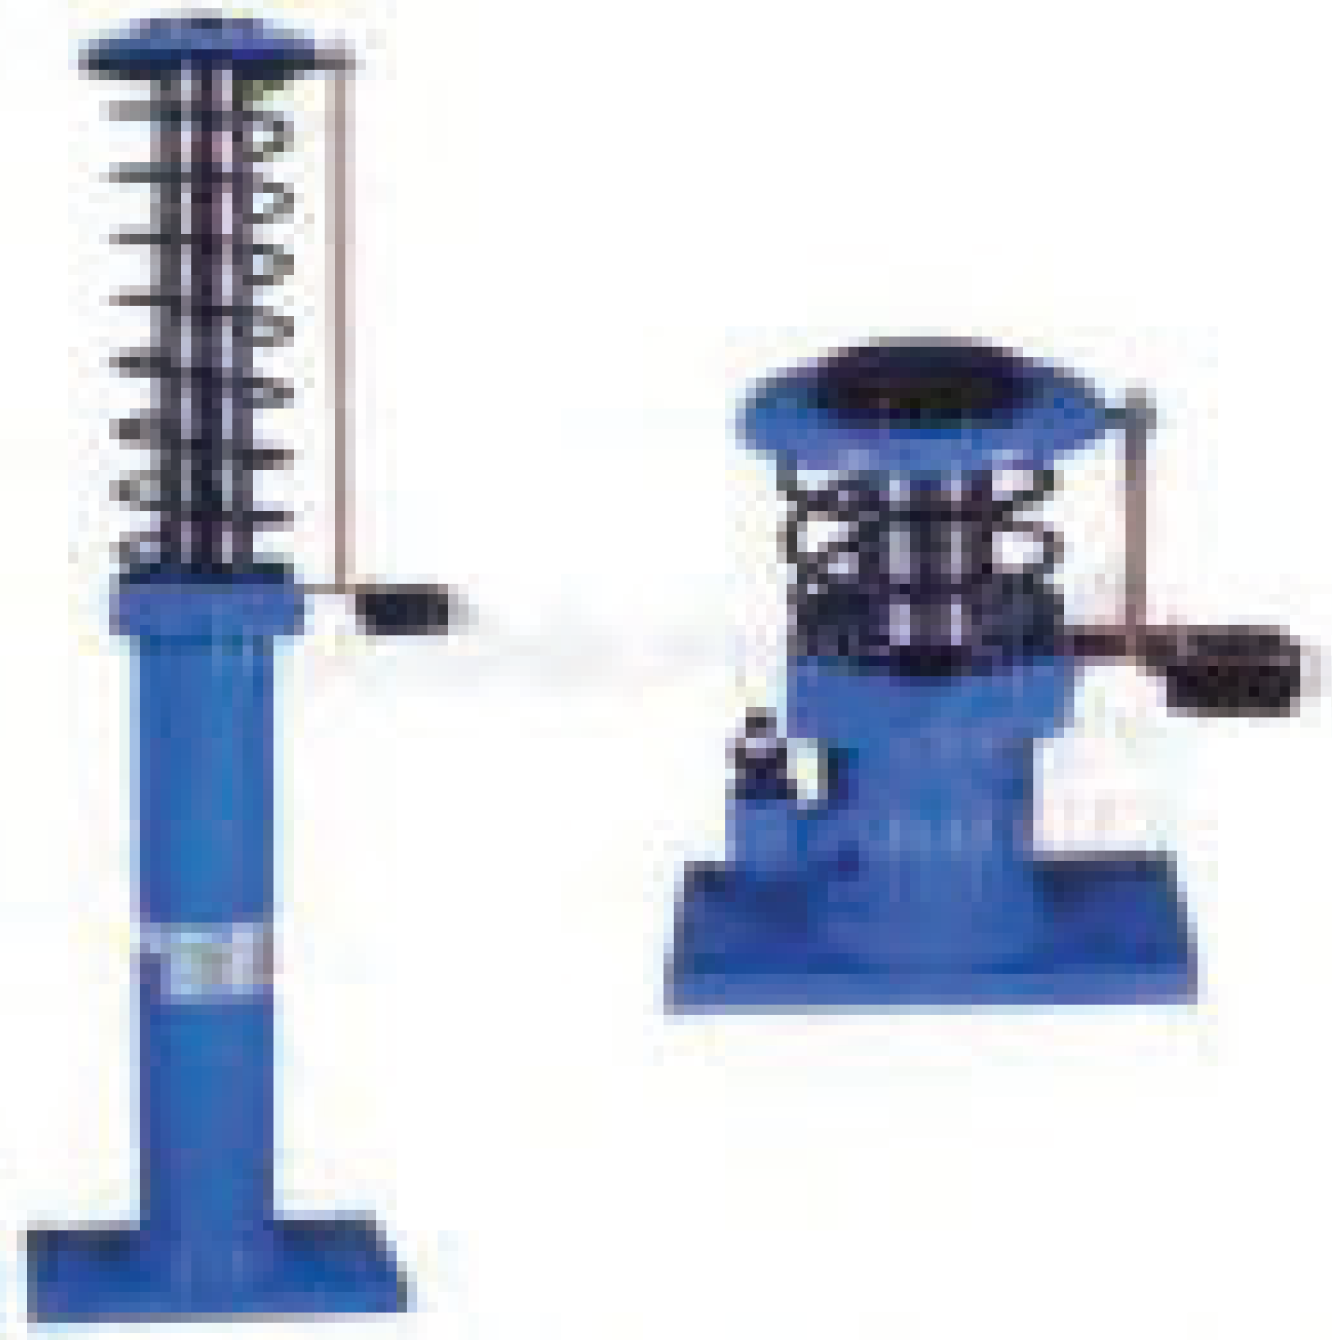
\includegraphics[width=0.35 \linewidth, keepaspectratio=true]{img/diagrams/elevator-buffer.png} %% , angle=90 trim={<left> <lower> <right> <upper>}
\caption{\label{fig:fig_elevator_buffer} \footnotesize{Buffers hidráulicos.}}
\end{center}
\end{wrapfigure}
%%\end{figure}

Planteamos además la condición que el ascensor tarde $1.6 \si[per-mode=symbol]{\second}$ en detener la cabina, valor que permite lograr una aceleración máxima aceptable, también se plantea a máxima carga y que el frenado se hará a aceleración lineal. Con estás consideraciones, se tiene que se alcanza una velocidad de caída de $-7.84 \si[per-mode=symbol]{meter\per\second}$ antes de que se accione el sistema de frenado y cayendo en ese lapso $3.136 \si[per-mode=symbol]{\meter}$, estos valores permitirán diseñar el buffer hidráulico para el peor caso.  Luego con estos valores y la condición de aceleración se plantea:


\begin{equation}
 \begin{cases}
 a_f{_{\left( t \right)}} = & A \cdot t + B \\
 v_f{_{\left( t \right)}} = &\frac{A}{2} \cdot t^2 + B \cdot t + C\\
 x_f{_{\left( t \right)}} = &\frac{A}{6} \cdot t^3 + \frac{B}{2} \cdot t^2 + C \cdot t + D\\
 v_{\left( t_{f} \right)} =& 0\\
 a_{\left( t_{f} \right)} =& g\\ 
 t_{f} = 1.6 \si[per-mode=symbol]{\second}  
 \end{cases} 
\end{equation}

De donde obtenemos:

\begin{empheq}[box={\mybluebox[5pt]}]{equation}
 \begin{cases}
 {x_{cmin}}_{\left( t \right)} = & 1.0203 \si[per-mode=symbol]{\meter\per\second\cubed} \cdot t^3 - 7.84 \si[per-mode=symbol]{\meter\per\second\squared} \cdot t - 3.136 \si[per-mode=symbol]{\meter} \\
 {v_{cmin}}_{\left( t \right)} = & 3.0625 \si[per-mode=symbol]{\meter\per\second\cubed} \cdot t^2 7.84 \si[per-mode=symbol]{\meter\per\second\squared}\\
 {a_{cmin}}_{\left( t \right)} = & 6.125 \si[per-mode=symbol]{\meter\per\second\cubed} \cdot t
 \end{cases} 
\end{empheq}


Donde la aceleración lineal implica una fuerza lineal por parte del motor para lograr este frenado.


\clearpage


\subsection{Resolución del problema numérico}

Para la resolución de la parte de programación del trabajo práctico e implementar los algoritmos pedidos, decidimos usar \textbf{MATLAB}, mayormente por conocerlo previamente y la sencillez con la que se pueden escribir scripts que implementen los algoritmos. A pesar de que la resolución se realizó en \textbf{MATLAB}, se prestó atención a la compatibilidad con \textbf{Octave}, ya que la compatibilidad en los paquetes básicos es alta y con un poco de cuidado y algo de programación condicional se puede lograr que los scripts funcionen en ambos entornos.
Todas las salidas numéricas se guardaron en archivos que luego fueron leídas en \LaTeX\space usando paquetes para el proceso de archivos en formato \textbf{\quotemarks{CSV}}, los mismos permiten redondeo, presentación y hasta algunas operaciones sobre los datos, lo cual facilita el escribir el informe de tal manera de que no deba modificarse al modificar los datos, basta con compilar nuevamente. Las imágenes en forma similar, se guardaron por código desde \textbf{MATLAB} en formato \textbf{\quotemarks{PNG}} y luego se incorporaron desde \LaTeX. Algo a mencionar es que se estimaron lo valores del orden de convergencia y la constante asintótica, para cada uno de el método numérico implementado.





\section{Gráficos de las funciones obtenidas para media carga}

A continuación se muestran las gráficas de las funciones de posición, velocidad y aceleración para media carga, $n_{personas} = 6$.


\begin{figure}[!h] %htb
\begin{center}
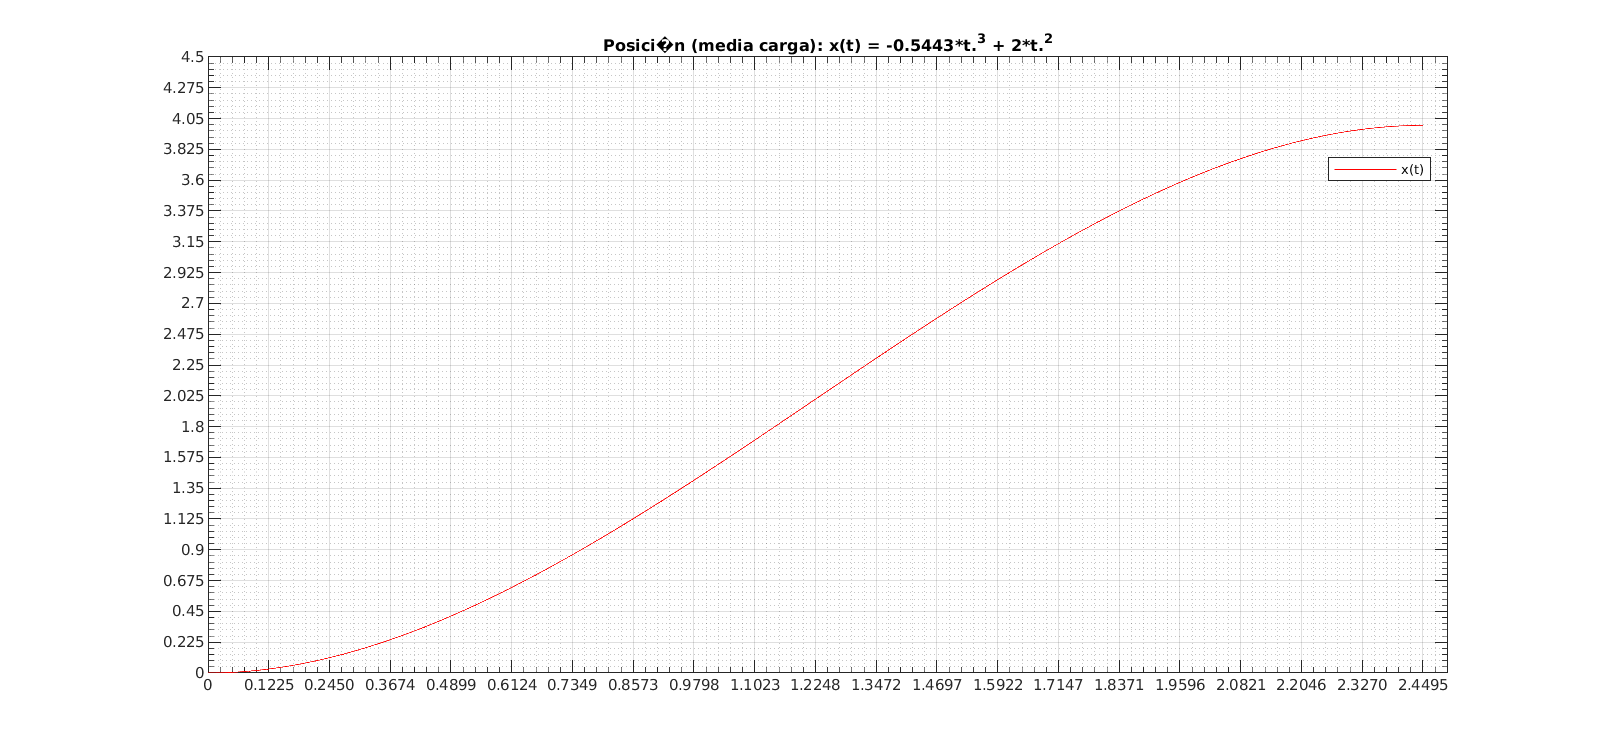
\includegraphics[width=1.2 \textwidth, keepaspectratio=true, angle=90]{img/grafico_funcion_x.png} %% , angle=90 trim={<left> <lower> <right> <upper>}
\caption{\label{fig:fig_position_n_2} \footnotesize{Posición en función del tiempo a media carga.}}
\end{center}
\end{figure}

\clearpage

\begin{figure}[!h] %htb
\begin{center}
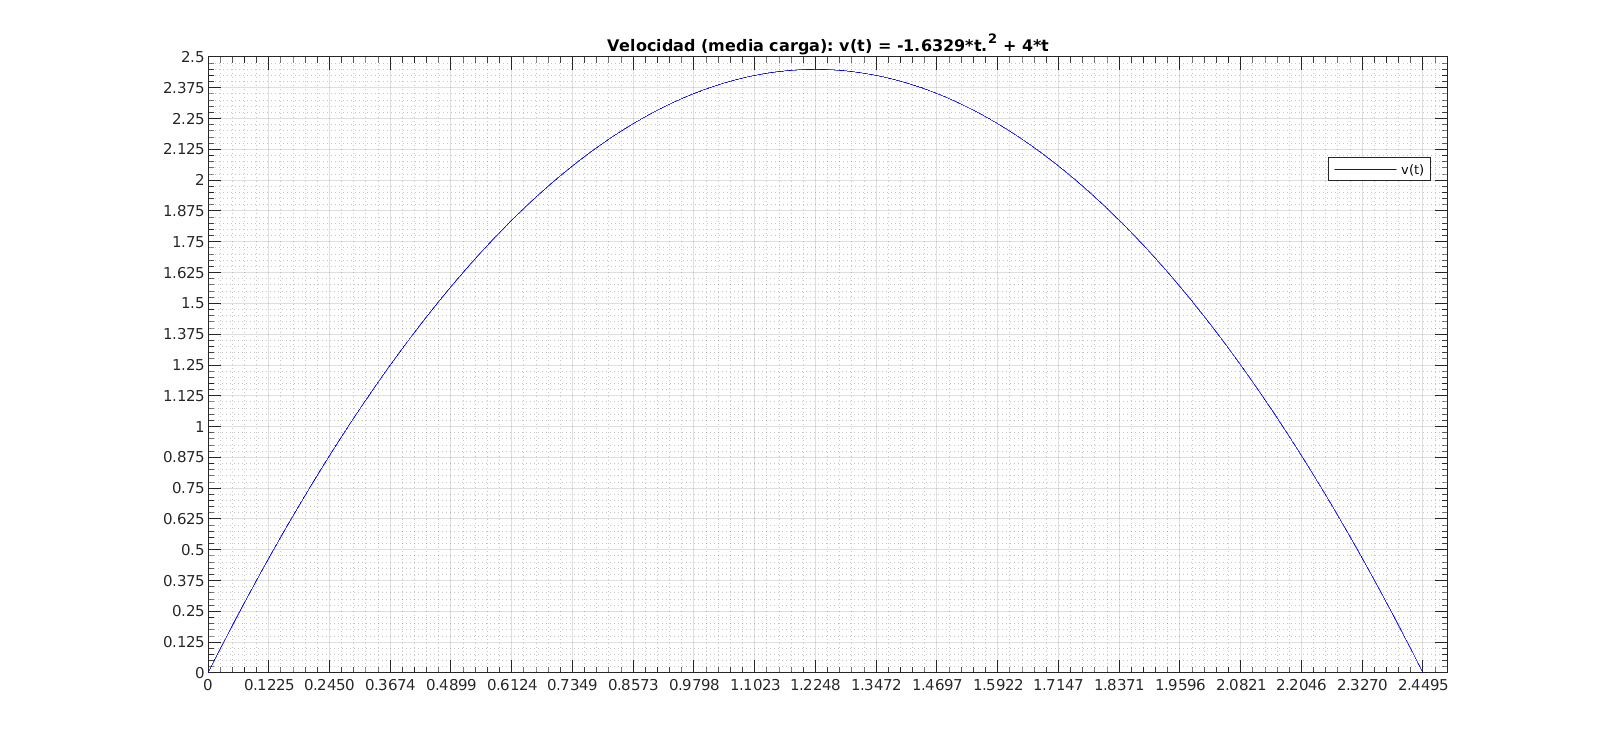
\includegraphics[width=1.2 \textwidth, keepaspectratio=true, angle=90]{img/grafico_funcion_v.png} %% , angle=90 trim={<left> <lower> <right> <upper>}
\caption{\label{fig:fig_position_n_2} \footnotesize{Valocidad en función del tiempo a media carga.}}
\end{center}
\end{figure}

\clearpage

\begin{figure}[!h] %htb
\begin{center}
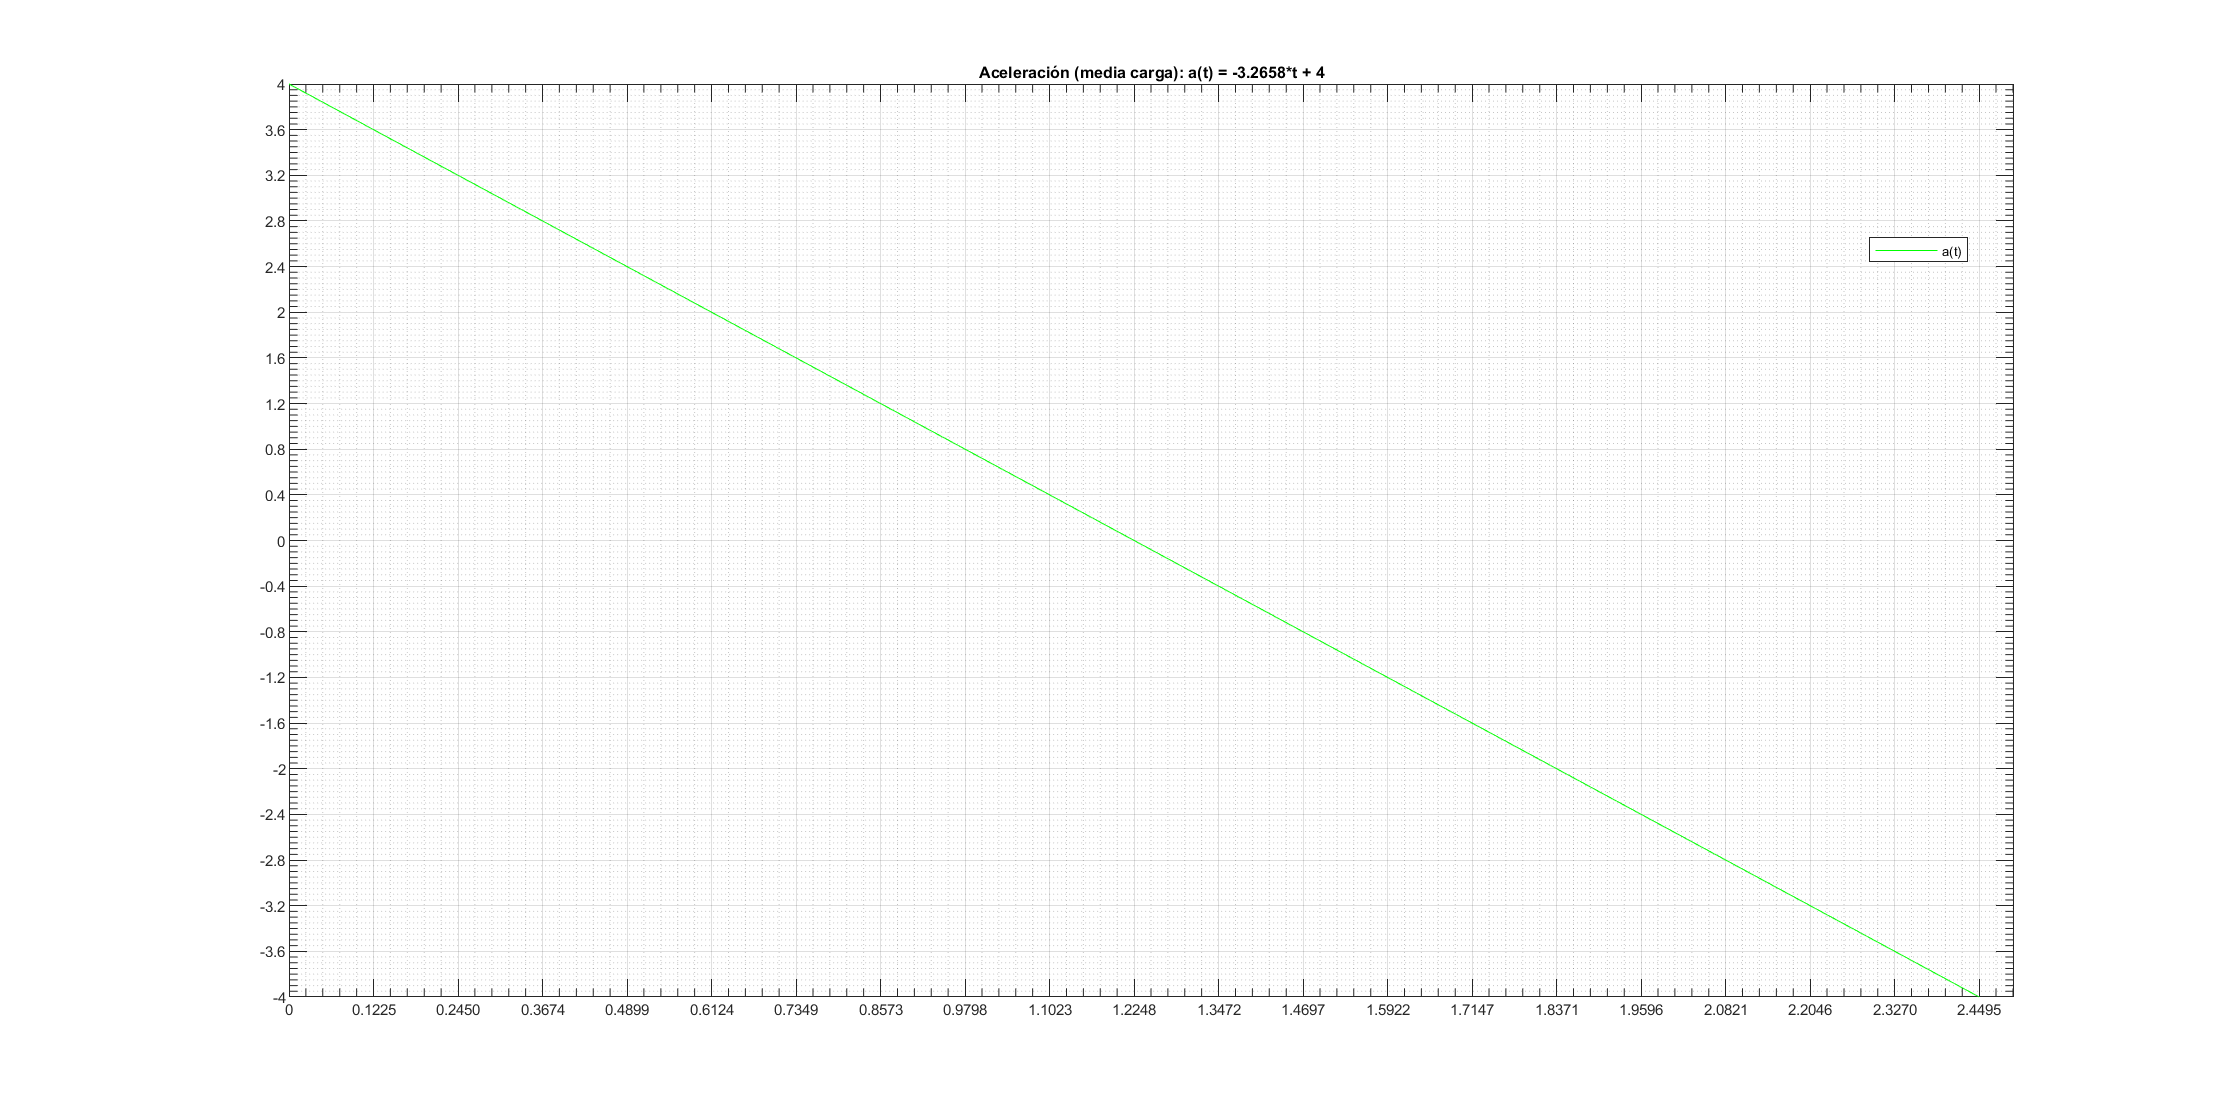
\includegraphics[width=1.2 \textwidth, keepaspectratio=true, angle=90]{img/grafico_funcion_a.png} %% , angle=90 trim={<left> <lower> <right> <upper>}
\caption{\label{fig:fig_position_n_2} \footnotesize{Aceleración en función del tiempo a media carga.}}
\end{center}
\end{figure}

\clearpage

